\documentclass{standalone}

\usepackage{graphicx}

\usepackage{tikz}

\usetikzlibrary{positioning}
\usetikzlibrary{arrows.meta}
\usetikzlibrary{calc}

\begin{document}

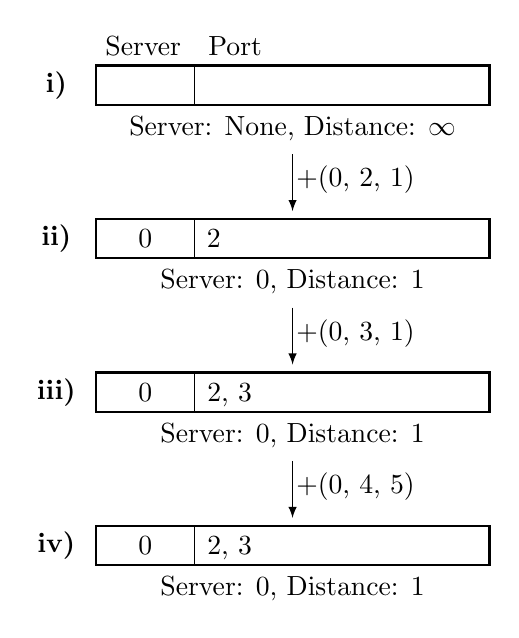
\begin{tikzpicture}[
    block/.style={align=center, rectangle, draw=black, fill=white, text width=16em}
]
    \node[] (T1) {Server};
    \node[] (T2) [right=0.1cm of T1] {Port};

    % Empty figure
    \node[] (H1) at (T1.south west) {};
    \draw[thick] ($(H1)+(0, 0.0)$) rectangle ($(H1)+(5,-.5)$);
    \draw ($(H1)+(1.26, 0.0)$) -- ($(H1)+(1.26,-.5)$);

    \node[] (I1) at ($(H1)+(-0.5, -.25)$) {\textbf{i)}};
    \node[] at ($(H1)+(2.5, -0.8)$) {Server: None, Distance: $\infty$};

    % After first addition
    \node[] (H2) [below=1.7cm of H1] {};
    \draw[thick] ($(H2)+(0, 0.0)$) rectangle ($(H2)+(5,-.5)$);
    \draw ($(H2)+(1.26, 0.0)$) -- ($(H2)+(1.26,-.5)$);

    \node[] at ($(H2)+(0.63, -.25)$) {0};
    \node[] at ($(H2)+(1.5, -.25)$) {2};

    \node[] (I2) at ($(H2)+(-0.5, -.25)$) {\textbf{ii)}};
    \node[] at ($(H2)+(2.5, -0.8)$) {Server: 0, Distance: $1$};

    % After second addition
    \node[] (H3) [below=1.7cm of H2] {};
    \draw[thick] ($(H3)+(0, 0.0)$) rectangle ($(H3)+(5,-.5)$);
    \draw ($(H3)+(1.26, 0.0)$) -- ($(H3)+(1.26,-.5)$);

    \node[] at ($(H3)+(0.63, -.25)$) {0};
    \node[] at ($(H3)+(1.7, -.29)$) {2, 3};

    \node[] (I2) at ($(H3)+(-0.5, -.25)$) {\textbf{iii)}};
    \node[] at ($(H3)+(2.5, -0.8)$) {Server: 0, Distance: $1$};

    % After final addition
    \node[] (H4) [below=1.7cm of H3] {};
    \draw[thick] ($(H4)+(0, 0.0)$) rectangle ($(H4)+(5,-.5)$);
    \draw ($(H4)+(1.26, 0.0)$) -- ($(H4)+(1.26,-.5)$);

    \node[] at ($(H4)+(0.63, -.25)$) {0};
    \node[] at ($(H4)+(1.7, -.29)$) {2, 3};

    \node[] (I2) at ($(H4)+(-0.5, -.25)$) {\textbf{iv)}};
    \node[] at ($(H4)+(2.5, -0.8)$) {Server: 0, Distance: $1$};

    % Transition indications
    \node[] (T2) at ($(H1)+(2.5, -1)$) {};
    \draw[-latex] (T2) -- ($(H2) + (2.5, 0.1)$);
    \node[] at ($(T2)+(0.8, -0.45)$) {+(0, 2, 1)};

    \node[] (T3) at ($(H2)+(2.5, -1)$) {};
    \draw[-latex] (T3) -- ($(H3) + (2.5, 0.1)$);
    \node[] at ($(T3)+(0.8, -0.45)$) {+(0, 3, 1)};

    \node[] (T4) at ($(H3)+(2.5, -1)$) {};
    \draw[-latex] (T4) -- ($(H4) + (2.5, 0.1)$);
    \node[] at ($(T4)+(0.8, -0.45)$) {+(0, 4, 5)};
\end{tikzpicture}

\end{document}